\section{Realisation}
Schon bei Projektstart wurde klar, dass es sich um sehr umfangreiche Anforderungen handelt. Es galt nicht nur eine Streaming Lösung zu implementieren, sondern es mussten auch alle Hardwarekomponenten getestet und angesteuert werden. Für die Bedienerseite musste eine funktionale Webseite einschließlich Webserver erstellt werden und ein Streaming-Server für die Konvertierung und Vernetzung der Sender und Empfänger musste konfiguriert werden. Viele \textbf{wichtige} bisher nicht genannte Anforderungen, z.B. Cybersicherheit, Authentifizierung wurden weitestgehend außer acht gelassen. Sie sind natürlich für eine endgültige industrielle Anwendung unerlässlich.\\

Das Projekt wurde in Teil-Aufgaben realisiert:
\begin{itemize}
\item Inbetriebnahme aller Hardwarekomponenten

\item Direktes Streamen von Audio und Video vom embedded System an PC
\item Aufsetzen eines Webservers im lokalen Netzwerk, lokales hosting der Webseite
\item Aufsetzen eines Streaming-Servers im lokalen Netzwerk
\item Direktes Streamen von Audio und Video vom embedded System an Streaming-Server
\item Anzeige des konvertierten Outputs des Streaming-Servers auf der Webseite

\item Streamen der PC Webcam an lokalen Streaming-Server
\item Zurück-Streamen vom Streaming-Server an embedded Hardware und Visualisierung

\item Hochladen der Webseite auf eine Online-Webspace
\item Aufsetzen eines Online-Streaming-Servers
\end{itemize}

\subsection{Inbetriebnahme der Hardware Komponenten}
Am Anfang des Projektes wurden alle Hardwarekomponenten bestellt und getestet. Raspberry PI B3+, Touchdisplays, Gehäuse, USB Lautsprecher, Webkameras mit Mikrofon und MMC Karten, siehe Lastenheft auf www.trello.com (Gruppe 15) für eine detaillierte Hardwareaufstellung. Danach kam die Installation des Betriebssystems RASPIAN auf den Raspberry PI3+ Boards und die Konfiguration eines Zugangs über SSH, siehe Kapitel \ref{RefRaspi}. Für Audio und Video Tests wurden *.mp4 Files und *.wav Dateien abgespielt, siehe Kapitel \ref{RefLautsprecher}. WLAN befindet sich bereits bei PI3+ als Komponente auf dem Board und musste nur konfiguriert werden. Die Mikrofon Tests gestalteten sich anspruchsvoller und es wurden Facebook Chat und WebRTC Internet Beispiele verwendet.

\subsection{Streamen vom embedded System > Server }
Um A/V Streaming auf dem Raspberry zu starten, wurden ffmpeg und gstreamer mit den 
vorkompilierten Paketen über den Paketmanager installiert. Wobei gstreamer den vollen Funktionsumfang (verglichen mit Ubuntu 18) hatte. Für Installationsanleitung und kompletter Liste der Testbefehle, siehe Kapitel \ref{RefGstreamer}. \\

Die Verwendung von ffmpeg gestaltete sich jedoch problematisch. Die Pakete des Paketmanagers unterstützten weder ffserver noch ffplay und es fehlten Abhängigkeiten zu diversen Bibliotheken. Es war nötig ffmpeg aus den Quellen zu bauen, siehe Kapitel \ref{RefFFmpeg} mit Schritt für Schritt Anleitung und alle durchgeführten Tests. Bei der Installation stellte sich heraus, dass ffserver nicht mehr in der aktuellen Version 4 unterstützt wird und es wurde via Git die Version 3.5 ausgecheckt. Dies bewirkte eine Kettenabhängigkeit der x264 Bibliothek, deren Version nun ebenfalls herunter gesetzt werden musste. Schließlich stand eine voll funktionsfähige ffmpeg, ffserver und ffplay Version bereit.\\ 

\textbf{Direktes Streamen von Audio und Video vom embedded System an PC}\\
Ffmpeg A/V Streaming hatte ein Delay von >2.5s, siehe Testergebnis \textbf{(m)} in Kapitel \ref{RefVergleich}. Der Stream wurde mit ffmpeg erzeugt und an den ffserver auf dem PC geschickt. ffplay, mplayer und vlc wurden ohne Verbesserung des Ergebnisses getestet.\\
Gstreamer konnte dieses Ergebnis bei weitem übertreffen. A/V Streaming ohne Server war nahezu ohne Verzögerung ca. 0.1s, siehe Testergebnis \textbf{(h)} in Kapitel \ref{RefVergleich}. Gstreamer erfüllte damit die Anforderung und wurde für im Projekt verwendet, um A/V direkt an den Streaming-Server zu senden. \\

\textbf{Aufsetzen eines Webservers im lokalen Netzwerk, Hosting der Webseite}\\
Als Webserver wurde nginx ausgewählt, um eine Webseite im lokalen Netzwerk zu hosten. Die Demo-Webseiten des Streaming-Servers benötigen noch diverse Anpassungen, um z.B. den Admin/Monitor verwenden zu können. Erst danach steht mit nginx eine vollwertige Entwicklungsumgebung zur Verfügung. Installation und Konfiguration von nginx wird in Kapitel \ref{Refnginx} erklärt. \\

\textbf{Aufsetzen eines Streaming-Servers im lokalen Netzwerk}\\
Die Auswahl einen OpenSoure Streaming Servers gestaltete sich schwierig. Mit der Anforderung einen A/V Stream im RTP/UDP Format in ein Web natives Format zu konvertieren und der geringen Anzahl veröffentlichter Projekte musste häufig die Dokumentation der Server zu Rate gezogen werden. In die engere Auswahl wurde UV4L und das Janus-Gateway gezogen. Die UV4L Bibliothek erwähnt zwar eine Einsatzmöglichkeit auch ohne Webbrowser. Es konnten jedoch keine Anwendungen gefunden werden, die UV4L zum direkten A/V Streaming verwenden.\\
Beim Janus-Gateway stand zumindest eine Standard-Konfiguration für RTP zu WebRTC bereit und in Foren werden Probleme nicht korrekter Konfiguration diskutiert. Auch ist das Empfangen von gstreamer RTP-Paketen möglich. Die Installation und Konfiguration des Janus-Gateways ist in Kapitel \ref{RefJanus} beschrieben.\\

\textbf{Direktes Streaming von Audio und Video vom embedded System an Streaming-Server}\\
Gstreamer Befehle für die Übertragung von A/V vom Raspberry an das Janus-Gateway sind in Kapitel \ref{RefGstrToJanus} aufgelistet.\\


\subsection{Webseite zur Anzeige der Videostreams}
Beschreibung...\\

\textbf{Anzeige des konvertierten Outputs des Streaming-Servers auf der Webseite}\\
blah blah blah\\

\subsection{Streamen von PC > Server > Anzeige auf embedded Sytem}
Beschreibung...\\

\textbf{Streamen der PC Webcam an lokalen Streaming-Server}\\
blah blah blah\\

\textbf{Zurück-Streamen vom Streaming-Server an embedded Hardware und Visualisierung}\\
blah blah blah\\

\subsection{Online Setup}
Beschreibung...\\

\textbf{Hochladen der Webseite auf eine Online-Wespace}\\

Hochladen der Webseite via Filezilla...\\

\textbf{Aufsetzen eines Online-Streaming-Servers}\\
blah blah blah\\

\textbf{Webserver Verbindungstest}\\
Im oberen Bereich ist der gstreamer Befehl mit dem Audio udpsink host...5000 und Video udpsink...5001. Wireshark detektiert ankommende Pakete im Webserver (ip 85.214.211.169) vom raspberry pi (ip 77.14.37.230) an den UDP Ports 5000 (Audio Paketgröße 451) und UDP 5001 (Video Paketgröße 894).\\

\begin{minipage}{\textwidth}
    \begin{center}
        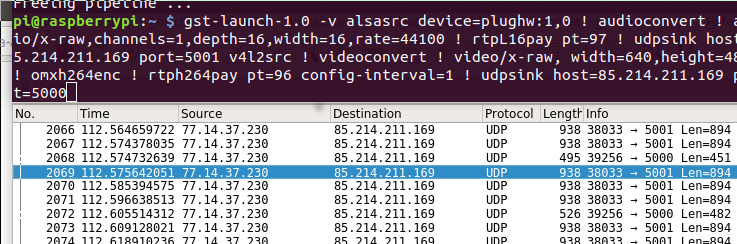
\includegraphics[scale=0.85]{img/wireshark.png} 
    \end{center}
\end{minipage}
